%%%%%%%%%%%%%%%%%%%%%%%%%%%%%%%%%%%%%%%%%%%%%%%%%%%%%%%%%%%%%%%%%
%                                                               %
%                       Legal Notice                            %
%                                                               %
% This document is copyright (C) Jason Gobat & Darren Atkinson	%
%                                                               %
%%%%%%%%%%%%%%%%%%%%%%%%%%%%%%%%%%%%%%%%%%%%%%%%%%%%%%%%%%%%%%%%%

\newpage{\pagestyle{empty}\cleardoublepage}

\chapter{Using {\em WinFElt}}
\label{winfelt}

\section{Introduction to {\em WinFElt}}
\label{winfelt.intro}

The primary feature of the main {\em WinFElt} window is a standard text
editor.    
\begin{figure}
\begin{center}
 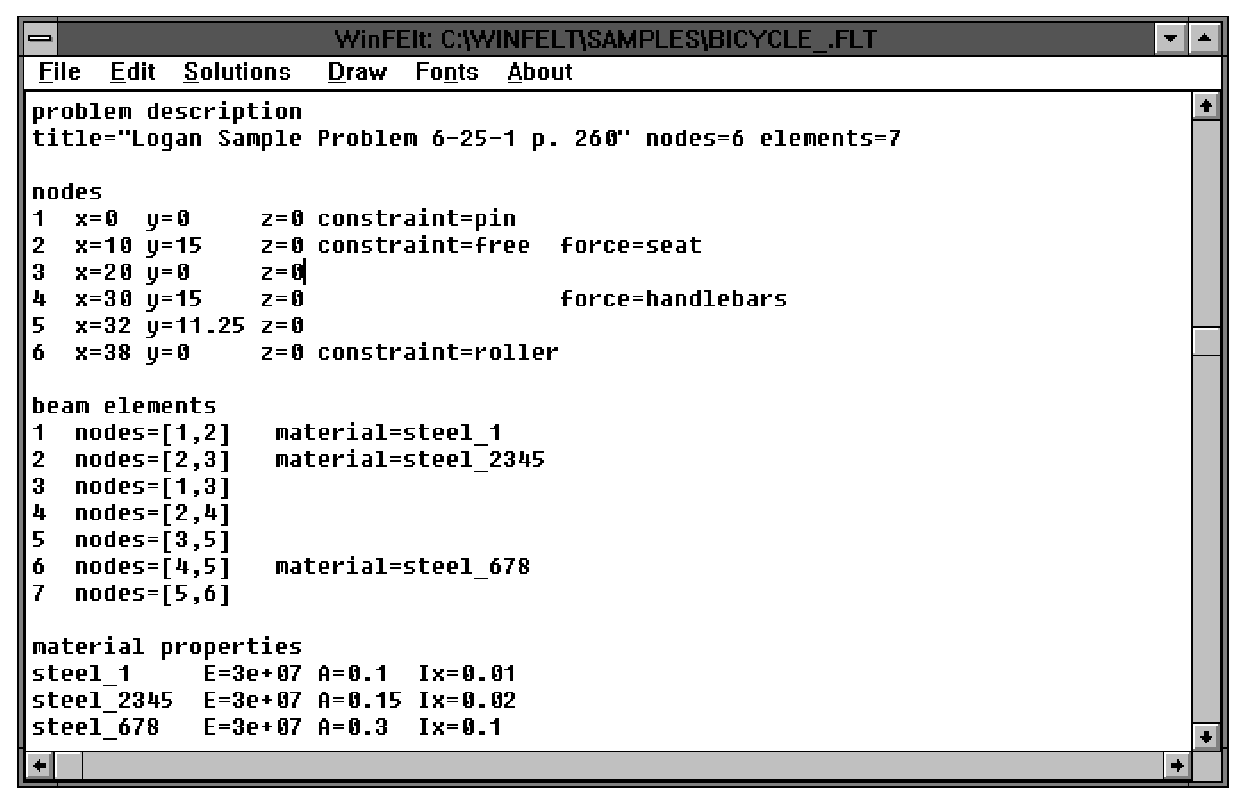
\includegraphics[width=5in]{figures/winfelt_main}
\end{center}
\caption{Main {\em WinFElt} editor with a sample problem.}
\label{winfelt.main}
\end{figure}

\section{Solving a problem}

Depending on what you want your solution to include, there are a couple
of different ways to go about solving a \felt{} problem from within
{\em WinFElt}.  In addition to the standard tabular type \felt{} output 
you can also have {\em WinFElt} generate
two-dimensional color shaded stress or displacement plots and/or plots 
of the structure with magnified displacements applied.  For transient 
analysis problems graphical time-displacement or time-temperature plots 
are available; in spectral analysis problems, plots of the transfer 
functions or ouput spectra are available.

All of the {\em WinFElt} output windows have a {\bf File} menu from
which you can save or print the results in that window.  
Line graphs are saved in Windows Metafile format (WMF) and
color contour plots are saved as Windows bitmaps (BMP)
Text output can be saved as an ASCII file.  Once an output window
is closed there is no way to bring the window back up without
resolving the problem.

One way to solve a problem is to select the {\bf solve} option from the
{\bf Solutions} menu.  By default, this simply generates the standard \felt{} 
tabular output in a text output window (figure~\ref{winfelt.output}). 
This window will contain either the mathematical solution of your problem 
or the syntax errors encountered in solving the problem.
%
\begin{figure}
\begin{center}
 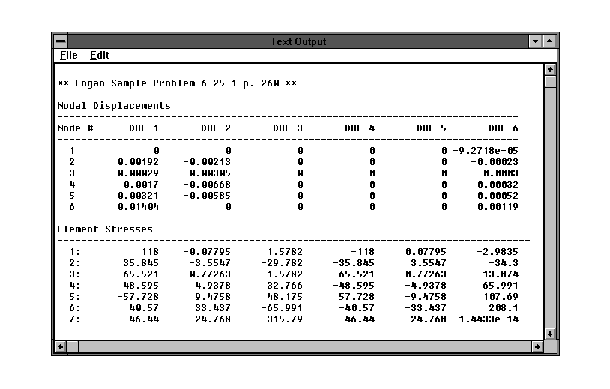
\includegraphics[width=5in]{figures/winfelt_output}
\end{center}
\caption{The text output box.}
\label{winfelt.output}
\end{figure}

For more control over what gets generated whenever you solve a problem
you can use the output control dialog box (figure~\ref{winfelt.controls}), 
available by selecting {\bf Controls} from the {\bf Solutions} menu.  
The toggle buttons and controls in this dialog box control all of the available
solution and output options, both text and graphical.   
%
\begin{figure}
\begin{center}
 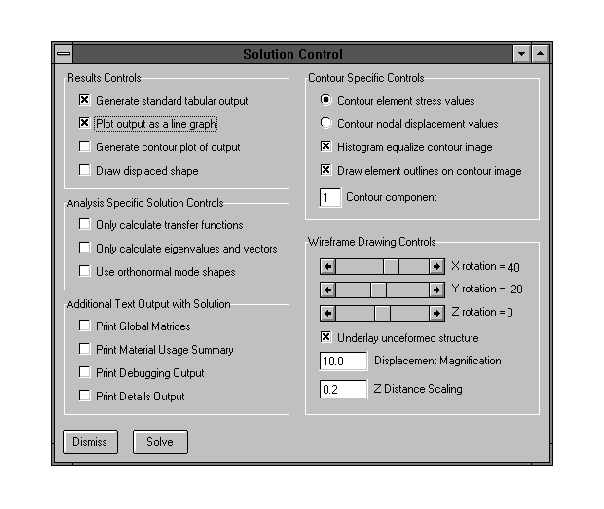
\includegraphics[width=4in]{figures/winfelt_controls}
\end{center}
\caption{The solution control box.}
\label{winfelt.controls}
\end{figure}

The toggles in the top-left corner determine the basic type of output
that you would like to generate -- tabular (available for all problem
types), line graphs (available for transient and spectral problems),
color contour plots (for static problems with planar elements), and
wireframe drawings (for static problem with any type of element).
If appropriate, multiple toggles can be selected for any given 
problem solution.

The next grouping of toggles are specific to spectral and modal analysis
and control exactly what types of results get generated during those
analyses.  

The final grouping of toggle buttons on the left side of 
figure~\ref{winfelt.controls} allows for the inclusion of 
ancillary information in the tabular text-based output.  Not all
of these toggle buttons will have an effect on solutions of
every analysis type -- for instance, global matrices are not
available in the solution of a nonlinear problem and the static
analyses currently do not print any details.

\section{Text output}

The text output from {\em WinFElt} is the most basic form of output that all 
applications in the \felt{} system produce.  That is, no matter how you specify
and solve a \felt{} problem (either with {\em felt},  
{\em velvet}, or {\em WinFElt}) the same kind of text output is available.
Chapter~\ref{felt_prog} details the interpretation of this basic output form.

\section{Graphical output}

\subsection{Contour plots}

The controls for color contour plots are available on the right side
of the main controls dialog (\ref{winfelt.controls}).
The two radio buttons control whether element stress or nodal
displacements are used as the basis for the interpolation.
For stress plots, the interpretation of the component number is element 
specific and must be a valid index in the stress vector for each element type 
in the problem.  Consult Table~\ref{felt_prog.stress_table} for details on 
what the stress vector consists of for each element type.  For displacement plots,
the component is simply the displacement DOF that you want to see plotted.
In general, this should be one of the active global DOF for the current
problem.

Other contouring controls include toggles for histogram equalization and
element boundary overlay.  Histogram equalization is a standard technique
in image processing for enhancing the contrast of images.  If the overlay
elements toggle is checked then the outline of all the elements in the problem
will be drawn in black on top of the color image.  An example of stress
contours (rendered here in greyscale) for the wrench example supplied with
{\em WinFElt} is shown in figure~\ref{winfelt.contour}.  Note that both histogram
equalization and element overlay were enabled for this plot.
\begin{figure}
\begin{center}
 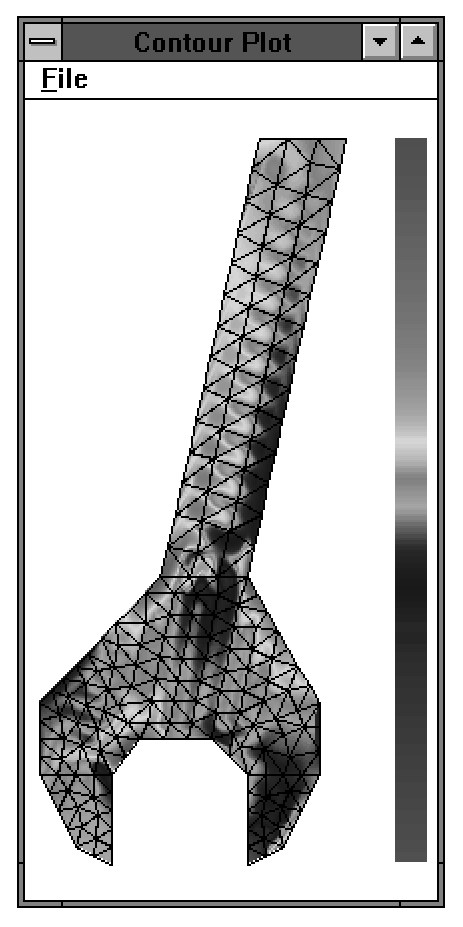
\includegraphics[width=3in]{figures/winfelt_contour}
\end{center}
\caption{A color contour plot showing the principal stress component in
         a static problem using constant strain triangular elements}.
\label{winfelt.contour}
\end{figure}

\subsection{Line graphs}

\begin{figure}
\begin{center}
 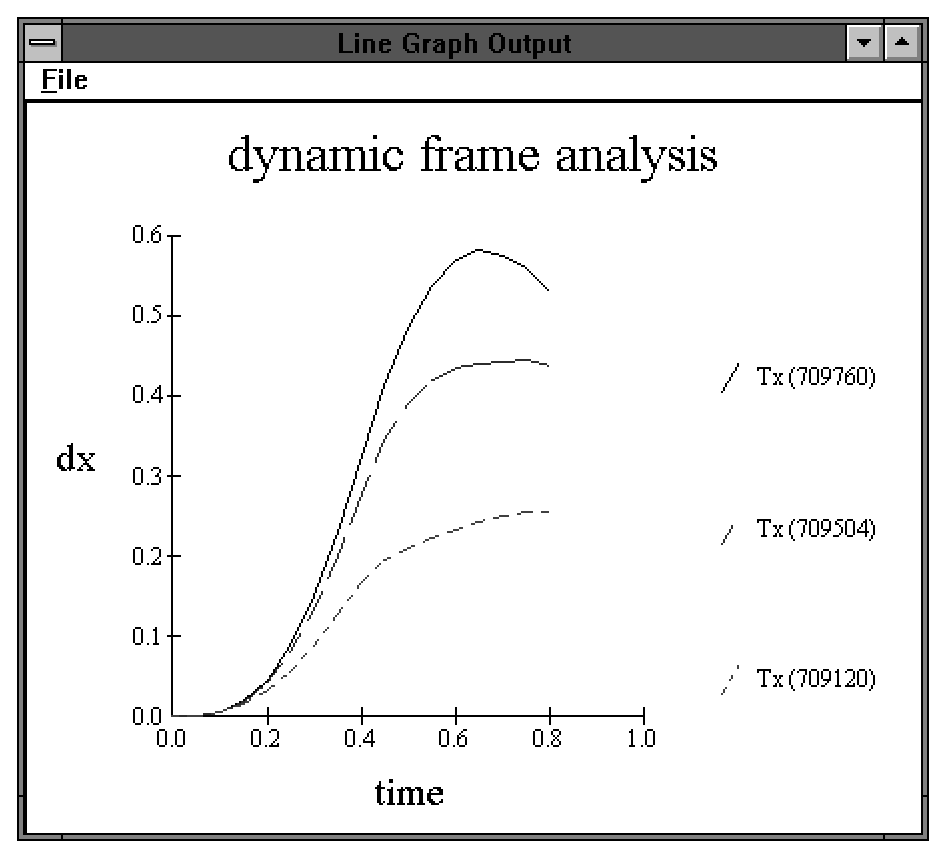
\includegraphics[width=4in]{figures/winfelt_graph}
\end{center}
\caption{A time-displacement plot in {\em WinFElt}}.
\label{winfelt.graph}
\end{figure}

\subsection{Wireframe drawings}

Most of the controls for wireframe drawing 
are specific to three-dimensional visualization.  The three sliders
control the rotation of the drawing about the three spatial axes.  The 
magnification determines the multiplicative factor by which nodal 
displacements will be increased before the nodes are plotted.  z scaling 
controls the front to back aspect ratio of the resulting plot.  

\begin{figure}
\begin{center}
 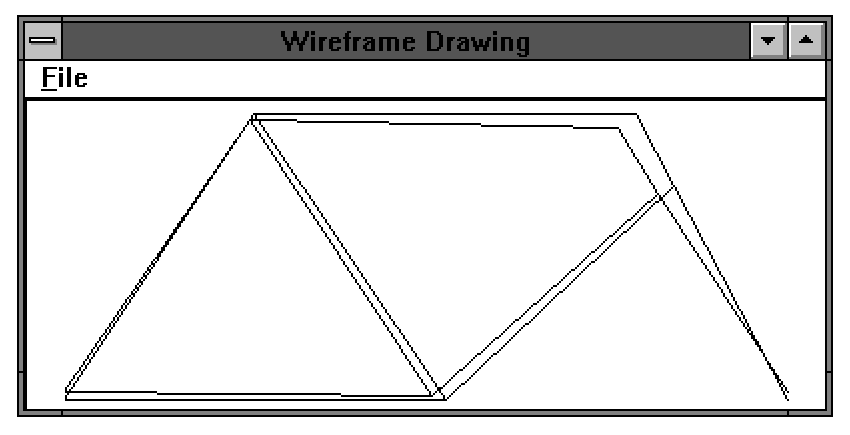
\includegraphics[width=4in]{figures/winfelt_wireframe}
\end{center}
\caption{An example of a displaced structure plot.}
\label{winfelt.wireframe}
\end{figure}

